%%% PREAMBLE - Do not touch %%%%%%%%%%%%%%%%%%%%%%%%%%%%%%%%%%%%%%%%%%%%%%%%%%%%%%
\documentclass[10pt,twocolumn,letterpaper]{article}
\usepackage[utf8]{inputenc}
\usepackage[portuges,brazil,english]{babel}
\usepackage{model}
\usepackage{times}
\usepackage{epsfig}
\usepackage{graphicx}
\usepackage{amsmath}
\usepackage{amssymb}
\usepackage{color}
\usepackage[pagebackref=true,breaklinks=true,letterpaper=true,colorlinks,bookmarks=false]{hyperref}

\cvprfinalcopy % *** Uncomment this line for the final submission
\def\httilde{\mbox{\tt\raisebox{-.5ex}{\symbol{126}}}}
\ifcvprfinal\pagestyle{empty}\fi

\newcommand{\TODO}[1]{TODO: #1}
\newcommand{\CITEONE}[2]{\mbox{#1 \cite{#2}}}
\newcommand{\CITETWO}[3]{\mbox{#1 and #2 \cite{#3}}}
\newcommand{\CITEN}[2]{\mbox{#1 et al. \cite{#2}}}

%%% Paper beginning %%%%%%%%%%%%%%%%%%%%%%%%%%%%%%%%%%%%%%%%%%%%%%%%%%%%%%%%%%%%%%
\begin{document}

%%% Title and authors %%%%%%%%%%%%%%%%%%%%%%%%%%%%%%%%%%%%%%%%%%%%%%%%%%%%%%%%%%%%
\title{MC886 - Trabalho prático 1}
\author{Guilherme P. Gonçalves (RA 091429)}

%%% Abstract %%%%%%%%%%%%%%%%%%%%%%%%%%%%%%%%%%%%%%%%%%%%%%%%%%%%%%%%%%%%%%%%%%%%%
\maketitle
\begin{abstract}
Este trabalho explora uma aplicação simples de técnicas de agrupamento de texto para categorizar emails. Um algoritmo é proposto, implementado e aplicado em um corpo de aproximadamente 18 mil emails.
\end{abstract}

%%% Introduction %%%%%%%%%%%%%%%%%%%%%%%%%%%%%%%%%%%%%%%%%%%%%%%%%%%%%%%%%%%%%%%%%
\section{Introdução}

Este trabalho explora técnicas de agrupamento de texto para classificar um corpo de emails por assuntos. O método, implementado em R, emprega o modelo tf-idf, que é comumente empregado para resolver problemas similares\cite{Steinbach00acomparison}, para gerar vetores descritores dos textos dos emails, e o algoritmo k-means para o agrupar esses vetores por assunto.

A Seção \ref{sec-problem} descreve o problema investigado por este estudo, enquanto a Seção \ref{sec-algorithm} descreve em detalhes a solução proposta. A Seção \ref{sec-experiments} contém os resultados experimentais da aplicação do algoritmo a um corpo de emails. Finalmente, a Seção \ref{sec-impl} apresenta alguns aspectos importantes de implementação não diretamente relacionados ao algoritmo.

\section{O problema analisado}
\label{sec-problem}

O problema explorado é uma aplicação simples de classificação de textos: dado um conjunto de 18828 textos de emails, analisá-los com um algoritmo de aprendizado de máquina de forma a descobrir quantos e quais assuntos eram neles abordados.

\section{Descrição do algoritmo}
\label{sec-algorithm}

Em uma descrição de alto nível, o algoritmo implementado possui duas fases: a construção do vetor de características para cada email e seu agrupamento.

Na fase de construção do vetor de características, os emails são lidos individualmente e divididos em \emph{tokens} separados por espaços. A seguir, os tokens são limpos através da remoção de alguns caracteres considerados ruído pelo algoritmo, tais como \_, =, $>$ e *. Essa limpeza tem dois propósitos principais: eliminar tokens compostos apenas por caracteres comumente usados por clientes de emails para indicar citações ou headers, e que portanto não carregam informação, e normalizar algumas variações da mesma palavra para um token só -- por exemplo, transformando ocorrências de "gray-scale" em "grayscale". Os tokens que ficam vazios após essa transformação são eliminados.

Os demais tokens são filtradas por um conjnunto de \emph{stopwords} em inglês, palavras muito comuns que pouco serviriam para classificar um email. As palavras restantes passam por um processo de \emph{stemming}, em que são reduzidas a sua forma raiz, novamente para compensar pequenas variações de grafia ou conjugação em palavras que deveriam ser a mesma. Tanto o processo de quebra em tokens quanto o stemming são feitos com o auxílio da biblioteca RWeka \cite{RWeka}.

O conjunto de todas as palavras únicas encontradas em todos os emails compõe o dicionário $D$ do problema. Para cada palavra $w$ do dicionário, contam-se o número de emails contendo aquela palavra, $ec[w]$:

\begin{displaymath}
ec[w] = |\{ d \in D : w \in d\}|
\end{displaymath}

Com isso, selecionam-se as palavras que serão de fato usadas como \emph{features} para descrever os vetores: enquanto os primeiros experimentos simplesmente selecionavam todas as palavras como features, restrições de memória e tempo de processamento levaram à escolha para features apenas das palavras que aparecem em mais de $1\%$ do total dos emails, o que reduz drasticamente o tamanho dos vetores de features resultantes e elimina diversas palavras de ruído que sobreviveram às etapas anteriores. 

Computado o conjunto de feature words $fw$, calcula-se para cada uma delas o \emph{inverse document frequency}, dado por:

\begin{displaymath}
idf[w] = \log{\frac{|E|}{ec[w]}}
\end{displaymath}

onde $E$ denota o conjunto de emails sendo analisados.

Para cada email e feature word, computa-se também o \emph{term frequency}, número de vezes que a feature word aparece no email:

\begin{displaymath}
tf[e, w] = count(w, e)
\end{displaymath}

O feature vector de um email é então dado pelo produto $tf[e] \times idf$, onde $tf[e]$ denota o vetor de $tf$ para as feature words naquele email. Os feature vectors são ainda normalizados para que tenham todos tamanho unitário, de forma a compensar pelos diferentes tamanhos dos emails.

Finalmente, na fase de agrupamento os feature vectors passam pelo algoritmo k-means para que os emails sejam divididos em \emph{clusters} por assunto em $k$ grupos. A Seção \ref{sec-experiments} contém mais detalhes sobre essa etapa, incluindo o processo de escolha do valor de $k$ pelo método do cotovelo.

Uma vez obtidos os clusters, deseja-se também determinar quais emails melhor representam cada um deles. Como o algoritmo k-means gera centróides dados por vetores que não necessariamente correspondem a um email, adotou-se como email centróide de cada cluster aquele de menor distância euclidiana ao centróide do cluster.

\section{Resultados experimentais}
\label{sec-experiments}

Esta seção contém os resultados experimentais da aplicação do algoritmo para um corpo de 18828 emails.

Para esses emails, construíram-se os feature vectors como na Seção \ref{sec-algorithm}. Foram utilizadas 1432 palavras como features, de forma que essa era a dimensão de cada feature vector. A título de ilustração, a Tabela \ref{tbl-feature-words} contém cinco feature words e os respectivos valores de idf.

\begin{table}
\begin{center}
\begin{tabular}{l*{6}{c}r}
Palavra & idf  \\
\hline
muslim & 3.9908979 \\
iron & 4.5960763 \\
specif & 3.0896625 \\
stuff & 2.9834855 \\
environm & 3.9794692 \\
\end{tabular}
\end{center}
\caption{Feature words e seus valores idf}
\label{tbl-feature-words}
\end{table}

A seguir, buscou-se um valor razoável de $k$ para o algoritmo k-means através do método do cotovelo. Nesse método, o faz-se k-means para diversos valores diferentes de $k$ e analisa-se um gráfico da distorção resultante, dada pela soma das distâncias de cada ponto ao centróide de seu respectivo cluster, para encontrar um valor $k^{*}$ em que a curva deixa de decrescer rapidamente, ou seja, a partir do qual adicionar clusters não descreve significativamente melhor os dados disponíveis. O valor $k^{*}$ assim encontrado é o valor mais adequado.

A fim de preservar recursos computacionais, e porque como parte da descrição problema sabia-se que o valor máximo de $k$ seria 100, fez-se a princípio uma busca grosseira para valores de $k$ variando de 2 a 100 de 5 em 5. A Figura \ref{fig-five-by-five} contém a curva de distorção para esse processo.

\begin{figure}
\begin{center}
	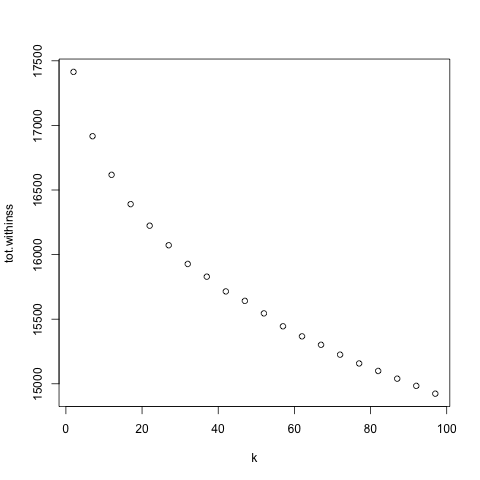
\includegraphics[width=0.99\columnwidth]{pics/five-by-five}
	\caption{Distorção do algoritmo k-means para k de 2 a 100, de 5 em 5.}
	\label{fig-five-by-five}   
\end{center} 
\end{figure}   

Uma abordagem parecida foi tentada utilizando como features palavras que apareciam em no mínimo $0.1\%$ em vez de $1\%$ dos textos. No entanto, o número adicional de features (nesse caso, 7473 palavras foram utilizadas) não trouxe diferença significativa no formato da curva, e apenas tornou o processamento proibitivamente mais caro no hardware disponível.

Embora não se observe na Figura \ref{fig-five-by-five} um "cotovelo" evidente, ela indica que a região inicial, para valores de $k$ abaixo de 50, deverá conter $k^{*}$. Para averiguar isso, fez-se a seguir um gráfico similar, desta vez para $k$ de 5 a 60, de 1 em 1. Esse gráfico pode ser visto na Figura \ref{fig-one-by-one}.

\begin{figure}
\begin{center}
	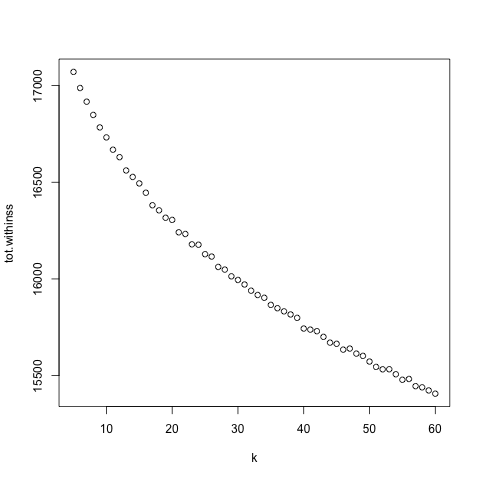
\includegraphics[width=0.99\columnwidth]{pics/one-by-one}
	\caption{Distorção do algoritmo k-means para k de 5 a 60, de 1 em 1.}
	\label{fig-one-by-one}   
\end{center} 
\end{figure} 

Novamente não se observa um "cotovelo" claro, mas da observação das Figuras \ref{fig-five-by-five} e \ref{fig-one-by-one} pode-se sugerir um valor de $k^{*} = 20$. O algoritmo k-means embutido na linguagem R foi então executado com um máximo de 100 iterações e 20 tentativas para os feature vectors e o valor escolhido de $k^{*}$. A Tabela \ref{tbl-centroids} mostra os centróides dos clusters obtidos dessa forma.

\begin{table}
\begin{center}
\begin{tabular}{l*{6}{c}r}
Cluster & Centróide \\
\hline
1 & eb2f9133b4b0bec6e81e1ed3fd6871ad.txt \\
2 & f21cc70562a389a74e140c1e40056297.txt  \\
3 & 29b01f5319a9856c1c4f09723773ec27.txt  \\
4 & af959473240dca5eccdb05302d0b8729.txt \\
5 & a9b0af073d3bb8077e12dc425b19a16d.txt \\
6 & 21c5def39d47ed609131635445d713f6.txt \\
7 & da29032bb3599fdfae59efaabeb0e00c.txt  \\
8 & 876a160d1de6899cf5a42f0ad14280ec.txt  \\
9 & d1612488548207a3a47843aa4b11946e.txt  \\
10 & 568dbca15836174d86fa49d6ae15759b.txt  \\
11 & 7c359f7b276c69a09f39de853613d661.txt  \\
12 & 00a8bead7c4c98afe18ce0dbbb1763a1.txt  \\
13 & 51fea6f8b25d31b044bc478f237ab2bc.txt  \\
14 & f1ecb5dcbc2c870130eb033074e5653e.txt \\
15 & 828542de06991d1aa4c175a574fde230.txt  \\
16 & 18b58765c5788629460ca2be1f5ae197.txt  \\
17 & 6c59d51c480725d6fc8b6efebcf6bbeb.txt   \\
18 & b958662c7fbe5a311db5a243a1bda205.txt  \\
19 & aa289fb4e31543bd4603c3ba8b181f6f.txt  \\
20 & 3ca6289ad6e0830ad81c57f0d0e573a0.txt  \\
\end{tabular}
\end{center}
\caption{Centróides para cada um dos clusters.}
\label{tbl-centroids}
\end{table}

O restante desta seção consiste em uma breve análise dos clusters obtidos, utilizando tanto o centróide quanto os três emails mais próximos dele.

A Tabela \ref{tbl-closest} contém os três emails mais próximos do centróide indicado na Tabela \ref{tbl-centroids} para cada um dos clusters.

\begin{table*}
\begin{center}
\begin{tabular}{ | l | l || l | l | p{8cm} |}
\hline
Cluster & Emails mais próximos & Cluster & Emails mais próximos \\
\hline
1 & \parbox[c][1.5cm]{6cm}{5b9632c4c3c57519facb45f2a5dd5a96.txt 71868b35bb0b811f7f5663f79a8c28ad.txt 0ee154d3e67ef3491d08c517bb6fe4df.txt} & 11 & \parbox[c][1.5cm]{6cm}{2755cab2f3e51f89ca0626c0a9abd270.txt 4c5e172dd2027a260ff57c97d445e0c8.txt d3defe1ce80c3e8e5f3690ff2de4bfd6.txt} \\
2 & \parbox[c][1.5cm]{6cm}{b2dc92abc4b68e5cdeb35387f8ed5f9d.txt 462269622ff446945d15b6d30654980c.txt 5a50f1acdd629680d3674615b9a338f7.txt} & 12 & \parbox[c][1.5cm]{6cm}{96b1a8d440f324d8f940eda1ad708688.txt 7a0b3d49a55a124dcc75c403420c0481.txt c522abec15bb519308450f94dfb40e3c.txt} \\
3 & \parbox[c][1.5cm]{6cm}{46d8a2cf039a2edd9fb76d8fe5b57a27.txt 2f95838d2fda44a43407c9e243e3384e.txt 72c8a757df1156692e96c7332737afd3.txt} & 13 & \parbox[c][1.5cm]{6cm}{36008db69e04ec4d33ede317ebc610e0.txt cc4d9d84fe5cf6c35ec8494274327f02.txt 2aabe5207a8473b97bd50e40f9edc05f.txt} \\
4 & \parbox[c][1.5cm]{6cm}{51f0c24f17369733f168eaeceac9ad8f.txt 2a14c92aad620ef59b6d0b87780f4814.txt decf2f483ed9c57954344fd6907ce901.txt} & 14 & \parbox[c][1.5cm]{6cm}{bdb3bc8a274e14e4502f451ecca48e1c.txt 5a84b4fdad31b7e2126f2e2666ec489d.txt cc3bf528d548f68f9a24035e52250c07.txt} \\
5 & \parbox[c][1.5cm]{6cm}{c0b40f790c6fce852050a1cd583b402e.txt 9268ca2ca808dfb3203493624d8de16d.txt c6d971c9a8a7e657850b2c02efe24b00.txt} & 15 & \parbox[c][1.5cm]{6cm}{aa9b5da52193ae6702e6bdb2b58c9689.txt d319f109965da97c9019c42eef7311e2.txt 6cd6904b27ee4c3fe30ca2f4ec328459.txt} \\
6 & \parbox[c][1.5cm]{6cm}{3ceb2061ab2d2c18bce8154a12992048.txt afa06f71e93f04f4a18e9093383b9dfe.txt 9eb334f10e9cc1ea237495af4b16179c.txt} & 16 & \parbox[c][1.5cm]{6cm}{c2237bdfcf99479a38c163d702129084.txt d3da10cf0cf00c4804340ff875a65ed4.txt 7f90830cc72af813b860f3507612d555.txt} \\
7 & \parbox[c][1.5cm]{6cm}{2adb9b7e74f340a7286f48ffee27c765.txt fcf4795a3ff768082c48123d3099228c.txt 9068f47025e17a92798bd6d501963f61.txt} & 17 & \parbox[c][1.5cm]{6cm}{063c99c35807c214821baf2322cd2a1f.txt c30b87a3cab64107d7645c7a3267a48e.txt 0ac219066196e61a5d6310599c39cb0b.txt} \\
8 & \parbox[c][1.5cm]{6cm}{933be2ef334f634b21ab972bbb3c7d5d.txt 6a60803a3f25cbf7afa977b0633fa784.txt 85686c1b3fcab0e81b51da08bbd80301.txt} & 18 & \parbox[c][1.5cm]{6cm}{78ee1bcf9ad28f01869e12cb8356b442.txt c2523343949c58ec7872a44890df9e90.txt 78787171952df493ac6df45743deb2a4.txt} \\
9 & \parbox[c][1.5cm]{6cm}{d14ca6250c73453f03f953fd4a932f91.txt 64bde302248786f3086758bad6eeed34.txt 437de825b1fc16f7214fb084d2bb8562.txt} & 19 & \parbox[c][1.5cm]{6cm}{3e9ddd1e7e87bac92ba60141d272112c.txt 44d6f3b22396ae4c3e38ba7c62bf76f3.txt 4719c3d122e0c7f65b672d8d62f92577.txt} \\
10 & \parbox[c][1.5cm]{6cm}{7beea049940fb8b12f43c48600abe1ec.txt 886483fadc2a405a5df48e7347bb037d.txt a8a044035ceee093af05f0c624fabdde.txt} & 20 & \parbox[c][1.5cm]{6cm}{61f339f0277cb05c595443666f7059e0.txt 341c946015fac9b47e9424e3b2d2cdd9.txt 3e4b63cf30a6c7c3b647f5f19274f62c.txt}  \\
\hline
\end{tabular}
\end{center}
\caption{Emails mais próximos do centróide para cada um dos clusters.}
\label{tbl-closest}
\end{table*}

Para o cluster 1, todos os emails destacados falam sobre armas e conflitos civis. Pode-se inferir que o cluster 1 se refere à discussão sobre porte de armas por civis. Dos emails do cluster 2, o centróide e dois dos emails mais próximos envolvem astronomia, mas o terceiro, presumivelmente classificado erroneamente, fala sobre privacidade na Internet.

Todos os emails selecionados do cluster 3 discorrem sobre hockey -- especificamente, sobre o ex-jogador e comentarista Don Cherry. Os emails do cluster 4 também todos abordam o mesmo tema, a religião cristã e discussões sobre a Bíblia.

Dos emails no cluster 5, 3 (incluindo o centróide) mencionam formatos de arquivos de imagens digitais, e o restante fala sobre formatos de arquivos em Mac. Presume-se assim que o tema desse cluster seja processamento de imagens. No cluster 6, todos os emails falam sobre implementação de interfaces gráficas, mencionando conceitos como gerenciadores de janelas.

Dentre os emails no cluster 7, dois, incluindo o centróide, falam sobre placas de vídeo, e os demais falam sobre outras placas de hardware -- a palavra "card" parece ser determinante aqui. Os emails do cluster 8 discorrem sobre compra de carros.

Dentre os emails do cluster 9, o centroide e dois dos mais próximos a ele versam sobre motocicletas, e o restante sobre "waterski bikes", um veículo marinho similar a uma motocicleta. No cluster 10 foram agrupados emails sem corpo, com apenas assunto ou mesmo sem assunto. O centróide, o único mais comprido, não possui assunto e apenas o texto \emph{"I AM Satan!"}.

Os emails do cluster 11 discutem conflitos étnicos e nazismo, enquanto os do cluster 12, embora abordem temas de tecnologia, não concordam em um tópico específico -- há emails sobre programação no sistema de janelas X, processos Unix, Windows 3.1 e programação em baixo nível.

Dos emails no cluster 13, três falam sobre hockey e um sobre baseball. Presumivelmente este cluster seria agregado ao cluster 3 em um experimento com $k$ menor.  Os emails do cluster 14 também abordam assuntos dispersos, como culinária, carros e processamento de imagens.

Os emails do cluster 15 falam sobre problemas de hardware em laptops, e os do cluster 16 discorrem sobre o conflito entre israelenses e palestinos. Os emails do cluster 17 discutem criptografia, e os do cluster 18 contém anúncios de vendas diversas.

Todos os emails do cluster 19 tratam de processamento de imagens, em uma possível concordância com o cluster 5. Finalmente, os emails do cluster 20 consistem em pessoas pedindo ou discutindo números de telefone.

Embora tenha-se observado alguma similaridade entre alguns pares de clusters, observa-se que o algoritmo proposto obteve resultados satisfatórios, em geral com todos os emails amostrados em cada cluster abordando os mesmos temas.

\section{Aspectos de implementação}
\label{sec-impl}

\section{Conclusão e melhorias futuras}
Present the main conclusions of the work as well as some future directions for other people interested in continuing this work. 

%%% References %%%%%%%%%%%%%%%%%%%%%%%%%%%%%%%%%%%%%%%%%%%%%%%%%%%%%%%%%%%%%%%%%%%
{\small
\bibliographystyle{unsrt}
\bibliography{references}
}

\end{document}
